
\documentclass[journal]{IEEEtran}
\usepackage[section]{placeins}
\usepackage{blindtext}
\usepackage{graphicx}
\usepackage{caption}
\usepackage{amsmath}
\usepackage{array}
\usepackage{url}

\ifCLASSINFOpdf
\else
\fi
\hyphenation{Gender Identification}


\begin{document}
	%
	% paper title
	\title{School of Engineering and Applied Science,Ahmedabad University\\Gender Identification}
	
	\author{Aatman Dholakia,~\IEEEmembership{1401013},
		Rajat Barot,~\IEEEmembership{1401045},
		Charvik Patel,~\IEEEmembership{1401079}, 
		Anuj Shah,~\IEEEmembership{1401084}}
	
	
	
	
	% make the title area
	\maketitle
	
	
	\begin{abstract}
		%\boldmath
		Machine Learning is being used widely in diverse areas such as fraudulent systems, recommender systems, disease prediction, etc. One such application is gender identification which is exploited in this paper. For gender identification it is necessary to extract features of face.The objective of this project is to identify the gender of a person by looking at his/her photograph. This is a case of supervised learning where the algorithm is first trained on a set of female and male faces, and then used to classify new data.We have not taken genders other than Male and Female into account 
		
	\end{abstract}
	\begin{IEEEkeywords}
		Face Detection, Gender Identification, SVM, Machine learning, classification algorithm, EigenFaces, K-Means
	\end{IEEEkeywords}
	
	
	\IEEEpeerreviewmaketitle
	
	
	
	\section{\textbf{Introduction}}
	Gender Identification has become area of extensive research due to it's increasingly powerful applications. Moreover augmenting it in real time scenario can be useful in many applications in many fields. A successful gender classification could have great impact in improving human computer interactions. Practically it is imperative to improve the algorithms from time to time in order to achieve higher accuracy levels and build more accurate and robust systems.In our Project We tried to identify gender from facial features, we are often curious about what
	features of the face are most important in determining gender.Are localized features
	such as eyes, nose and ears more important or overall features such as head shape,
	hairline, face contour and many more.\\
	In our Project Following Method are implemented for an classification Problem 
	\begin{enumerate}
		\item Eigenface Method
		\item K-Mean
		\item SVM
	\end{enumerate}
	
	
	
	
	
	
	
	\ifCLASSOPTIONcaptionsoff
	\newpage
	\fi
	
	
	
	\section{\textbf{METHODOLOGY}}
	Our proposed face detection and sex classification system is
	described in Fig. 1.\\
	\begin{minipage}{\linewidth}
		\centering
		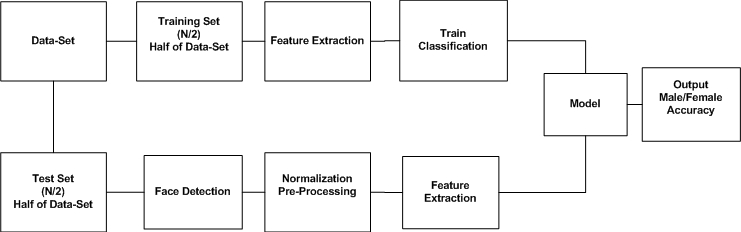
\includegraphics[width = 80mm,height=40mm]{Methodology.JPG}
		\captionof{figure}{Methodology \label{overflow}}
	\end{minipage} 
	\section{\textbf{Previous Approach}}
	\subsection{\textbf{Face Detection}}
	The proposed algorithm first locates the face region
	using skin-color. The YCbCr color space is used to detect
	the skin region on the given input face image. The given
	input RGB image is converted into the YCbCr color
	space.
	
	
	Color is a powerful cue of human faces. The
	distribution of skin clusters is in a small region of the
	chromatic color space. Processing color is faster than
	processing other facial features. Therefore, skin color
	detection is firstly performed on the input color image to
	reduce the computational complexity.
	
	In the color detection process, each pixel is classified as
	either skin or non-skin based on its color components.
	\begin{equation}
	GammaRGB=(c1*inputRGBimage)^{c21} + c3
	\end{equation}
	
	where $c1=1.0$, $c2=1.0$ and $c3=0.0$\vspace{1mm}\\
	
	The Y, Cb and Cr components are determined through
	the following formula using the constant C with the value
	128. $^{[1]}$
	\begin{equation}
	\begin{split}
	Y=(0.299*(gammaRGB[0,i,j]-C)+C\\
	+(0.114*(gammaRGB[2,i,j]-C)))
	\end{split}
	\end{equation}
	
	\begin{equation}
	\begin{split}
	Cb=(0.564*(gammaRGB[2,i,j]-Y)
	\end{split}
	\end{equation}
	
	
	\begin{equation}
	\begin{split}
	Cr=(0.713*(gammaRGB[0,i,j]-Y)
	\end{split}
	\end{equation}
	
	here, gammaRGB is the array with 0 represents the Red
	layer and the 2 represents the Blue layer. The range of Cb
	is between -50 and 2 while the range of Cr is between 10
	and 100 determine the skin region.The skin image is estimated based on the threshold
	gray level between 20 and 80.
	
	\subsection{\textbf{Facial feature Detection}}
	\begin{enumerate}
		\item Edge detection is done using Gabor's algorithm which implements linear approach..
		\item A set of Gabor filters with different frequencies and orientations may be helpful for extracting useful features from an image.
		\item In the discrete domain, two-dimensional Gabor filters are given by,\\
		\begin{equation}
		G_c[i, j] = Be^{(-(x^2+y^2)/2\sigma^2)}cos(2\pi f(icos\theta + jsin\theta))
		\end{equation}
		\begin{equation}
		G_s[i, j] = Ce^{(-(x^2+y^2)/2\sigma^2)}sin(2\pi f(icos\theta + jsin\theta))
		\end{equation}
		where B and C are normalizing factors to be determined and f is the frequency being looked for in the texture. $\theta$ is the direction in which feature is to be looked for.
	\end{enumerate}
	
	
	\section{Dataset}
	\begin{enumerate}
		\item Label our Data set
		\begin{enumerate}
			\item m = male
			\item f = female
		\end{enumerate}
		
		\item Dimension is 48 * 48 pixel
		
		
	\end{enumerate}
	\section{SVM}$^{[5]}$
	Support Vector Machine” (SVM) is a supervised machine learning algorithm which can be used for both classification or regression challenges.
	we perform classification by finding the hyper-plane that differentiate the two classes very well.
	\begin{minipage}{\linewidth}
		\centering
		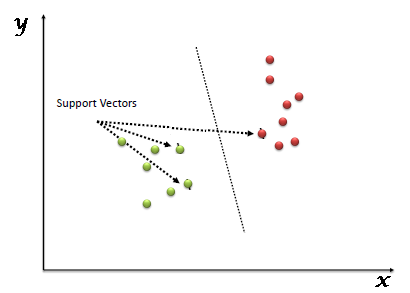
\includegraphics[width = 80mm]{svm1.png}
		\captionof{figure}{SVM-1 \label{overflow}}
		\end{minipage} 
	\begin{enumerate}
		\item You need to remember a thumb rule to identify the right hyper-plane: “Select the hyper-plane which segregates the two classes better”
		\item  maximizing the distances between nearest data point (either class) and hyper-plane will help us to decide the right hyper-plane. This distance is called as Margin.
		\begin{minipage}{\linewidth}
			\centering
			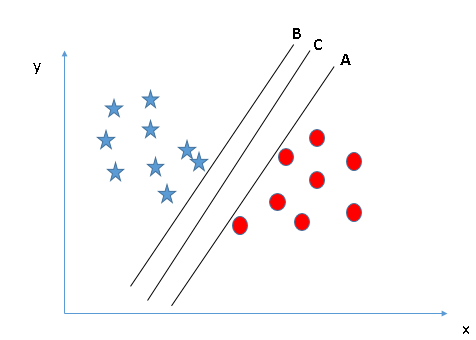
\includegraphics[width = 80mm]{svm2.png}
			\captionof{figure}{SVM-2 \label{overflow}}
		\end{minipage} 
		\item SVM has a feature to ignore outliers and find the hyper-plane that has maximum margin
		\item We have used sklearn library for SVM in python.
		
		
	\end{enumerate}	
	


	
\begin{center}
		\begin{tabular}{||c c ||} 
		\hline
		Gender & Error \\ 
		\hline\hline
		Male &   0.47\\ 
		\hline
		Female &   0.53\\
	\end{tabular}\\
	\small Table-1 SVM for Dataset-1
\vspace{0.5cm}\\
\begin{tabular}{||c c c c||} 
	\hline
	Class Label & Precision & Recall & F1-Score \\ 
	\hline\hline
	Male & 0.88 & 0.88 & 0.88 \\ 
	\hline
	Female & 0.74 & 0.75 & 0.743 \\ 
	\hline
	Avg/Total & 0.81 & 0.81 & 0.81 \\ 
	
\end{tabular}\\
	\small Table-3 For Precision,Recall,F1 Score,Support
		\vspace{0.5cm}
		
	\begin{tabular}{||c c c ||} 
		\hline
		Class Label & Male & Female \\ 
		\hline\hline
		Male & 176 & 24  \\ 
		\hline
		Female & 23 & 70  \\
	\end{tabular}\\
	\small Table-4 Confusion Matrix

\end{center}
\section{EigenFaces}
	Eigenfaces is the name given to a set of eigenvectors when they are used in the computer vision problem of human face recognition.the presence of some
	objects (eyes, nose, mouth) in any face as well as relative distances between
	these objects. These characteristic features are called eigenfaces in the facial
	recognition domain (or principal components generally). They can be extracted
	out of original image data by means of a mathematical tool called Principal
	Component Analysis (PCA).  The eigenvectors are derived from the covariance
	matrix of the probability distribution over the high-dimensional vector space of
	face images.	
	
		
		\begin{center}
			\begin{tabular}{||c c ||} 
				\hline
				Gender & Error \\ 
				\hline\hline
				Male & 0.64  \\ 
				\hline
				Female & 0.66  \\
			\end{tabular}\\
			\small Table-1 EigenFaces for Dataset-1
			\vspace{0.5cm}\\
			\begin{tabular}{||c c c c||} 
				\hline
				Class Label & Precision & Recall & F1-Score \\ 
				\hline\hline
				Male & 0.73 & 0.2 & 0.313 \\ 
				\hline
				Female & 0.33 & 0.84 & 0.47 \\ 
				\hline
				Avg/Total & 0.53 & 0.52 & 0.39 \\ 
				
			\end{tabular}\\
			\small Table-2 For Precision,Recall,F1 Score,Support
			\vspace{0.5cm}
			
			\begin{tabular}{||c c c ||} 
				\hline
				Class Label & Male & Female \\ 
				\hline\hline
				Male & 66 & 134  \\ 
				\hline
				Female & 60 & 33  \\
			\end{tabular}\\
			\small Table-3 Confusion Matrix
			
		\end{center}
		
	
	\section{K-Means}
	k-means is  one of  the simplest unsupervised  learning  algorithms  that  solve  the
	well  known clustering problem.  The  main  idea  is to define k centers, one for
	each cluster. These centers  should  be placed in a cunning  way  because
	of  different  location  causes different  result. this  algorithm  aims at  minimizing  an
	objective function know as squared error function given by:
	$$ J(v)= \sum_{i=1}^{c} \sum_{i=1}^{c_i} (\parallel x_i - v_j \parallel)^2$$
	Where,\\
	$\parallel x_i - v_j \parallel$: Euclidean Distance\\
	$c_i$: number of data point in $i^{th}$ Cluster\\
	$c$: number of cluster centers
	
		
		\begin{center}
			\begin{tabular}{||c c ||} 
				\hline
				Gender & Error \\ 
				\hline\hline
				Male & 0.79  \\ 
				\hline
				Female & 0.16  \\
			\end{tabular}\\
			\small Table-1 K-Means for Dataset-1
			\vspace{0.5cm}\\
			\begin{tabular}{||c c c c||} 
				\hline
				Class Label & Precision & Recall & F1-Score \\ 
				\hline\hline
				Male & 0.63 & 0.68 & 0.77 \\ 
				\hline
				Female & 0.61 & 0.66 & 0.75 \\ 
				\hline
				Avg/Total & 0.64 & 0.67 & 0.76 \\ 
				
			\end{tabular}\\
			\small Table-2 For Precision,Recall,F1 Score,Support
			\vspace{0.5cm}
			
			\begin{tabular}{||c c c ||} 
				\hline
				Class Label & Male & Female \\ 
				\hline\hline
				Male & 40 & 160  \\ 
				\hline
				Female & 15 & 78  \\
			\end{tabular}\\
			\small Table-3 Confusion Matrix
			
		\end{center}
	
	\section{\textbf{Conclusion}}
	For the Proper Gender Identification we need to Detect the face and need to detect the skin color,facial feature extraction,Geometric Distance between Extracted Feature and need to classify data into two class as follow
	\begin{enumerate}
		\item Male
		\item Female
	\end{enumerate} 
	\textbf{Eigenfaces}
	\begin{enumerate}
		\item Advantages:the algorithm is basically identifying almost every new face to be male, hence contributing to the large error for females.
		\item Disadvantages:it cannot give you an intuitive sense of why the algorithm is favouring males. But upon looking at the data where the algorithm misclassified the person, we conclude that female subjects who have short hair, hair tied back or in a scarf were almost always labeled male. Having insufficient examples for them to train on might have resulted in this outcome.
	\end{enumerate}
	\textbf{K-Mean$^{[6]}$}
	\begin{enumerate}
		\item Advantages:Faster then EigenFaces if variable are huge.
		\item Disadvantages:Running time is too slow since it compute distance between each of the k nearest point
	\end{enumerate}		
	\textbf{SVM}
	\begin{enumerate}
		\item Advantages: Computationally better then Eigenfaces and K-Means 
		\item Disadvantages:When Dimension are very high  then SVM result into large in-accuracy.
	\end{enumerate}
	
	
	
	
	\section{\textbf{Future Work}}
	\begin{enumerate}
		\item Train classifier to train images for gender classification i.e. person is male or female.
		\item To detect gender of more than one person in real time video at the same time.
		
		
	\end{enumerate}
	
	
	\begin{thebibliography}{1}
		\bibitem{IEEEhowto:kopka}
		“Digital Image Processing”, William K Pratt, Wiley
		Publication, 3rd edition.
		\bibitem{IEEEhowto:kopka}
		"Face Detection with Facial Features and Gender Classification Based On
		Support Vector Machine",S.Ravi,S.Wilson,[publication:2010]
		\bibitem{IEEEhowto:kopka}
		"Gender Detection using Machine Learning Techniques
		and Delaunay Triangulation",Sarthak Gupta[publication:August,2013]
		\bibitem{IEEEhowto:kopka}
		"Face Detection and Sex Identification from Color Images
		using AdaBoost with SVM based Component Classifier",Hafizur Rahman,Tonmoy Das,Manamatha Sarnaker[Publication:August,2013]
		
		\bibitem{IEEEhowto:kopka}
		Sunil Ray, "Understanding Support Vector Machine Algorithm From Examples (Along With Code)". Analytics Vidhya. \url{https://www.analyticsvidhya.com/blog/2015/10/understaing-support-vector-machine-example-code/}, 2017. Web. 11 Apr. 2017.
		\bibitem{IEEEhowto:kopka}
		tarun gulyani,"K-Means Clustering Advantages And Disadvantages". Playwidtech.blogspot.in. \url{http://playwidtech.blogspot.in/2013/02/k-means-clustering-advantages-and.html}, 2017. Web. 8 Mar. 2017.
		\bibitem{IEEEhowto:kopka}
		"Advantages and disadvantages of SVM",\url{https://core.ac.uk/download/pdf/6302770.pdf}
		\bibitem{IEEEhowto:kopka}
		Presision,recall and F1 score,\url{http://www.kdnuggets.com/faq/precision-recall.html}
		
	\end{thebibliography}
	
	
	
\end{document}


